%!TEX root = project.tex

\chapter*{About this project}

\paragraph{Abstract}


\paragraph{Authors}


\chapter*{Acknowledgements}


\chapter{Introduction}
\par Par

\par Test Par end reference\cite{NameOfreff}.

\chapter{Context}

\section{Objectives}
The overall objective of our project:

\begin{enumerate}
    \item \textbf{Objective1} About objective:
    \begin{itemize}
        \item Database 
        \item Authentication 
    \end{itemize}
    \item \textbf{Objective 2} The description and so on.
\end{enumerate}

\section{Project Links}
Links to this document.

\paragraph{Links}
\begin{itemize}
\item https://github.com
\item https://github.com
/
\end{itemize}

\section{Chapters Review}
Description of chapters

\subsection{Methodology}
Description of chapters

\subsection{Technology Review}
Description of chapters

\subsection{System Design}
Description of chapters

\subsection{System Evaluation}
Description of chapters

\subsection{Conclusion}
Description of chapters

\chapter{Methodology}
Description of chapters

\section{Agile Development}
aaaaaaaaaaaaaaaaaaaaaaaaaaaaaaaaa\par
blabla\cite{FirstnameLastname}.\par
bbbbbbbbbbbbbbbbbbbbbbbbbbbbbbbbbb\cite{NameOfreff}.

\section{Testing}
tttttttttttttttttttttttttttttt
\cite{FirstnameLastname}.


\chapter{Technology Review}
tehhhhhhhhhhhhhhhhhhhhhhhhhhhhhhh

\section{Development Environment}
different programming tools


\subsection{GitHub}

Some sample git commands used are as follows:
\begin{itemize}

    \item git add .\par
    Add folders .....

\end{itemize}

\subsection{Ionic}
Ionic is a framework with a stunningly designed graphical interface, styled for various platforms, for maximum similarity to native applications. AngularJS and sass are taken as a basis for the framework, AngularJS and sass are taken, which brought him great popularity among developers, as these technologies reduce the threshold of entry to a minimum. The core of the framework is Cordoba, so all the plugins of Cordoba will work fine on ionic.\par In addition to the platform and ready-made UI components, Ionic has a thoughtful command line interface that allows you o generate icons, splash screens, run the file in the browser with the app for debugging, and build applications with short commands in the console.\par Also worth noting is the detailed documentation with examples.\cite{Ionic}

\subsubsection{Ionic UI}
Ionic has dozens of ready-made components, which are constantly being refined and replenished with new ones. You can fully read them on the documentation page.\cite{IonicUI}

\begin{figure}[h]
\centering
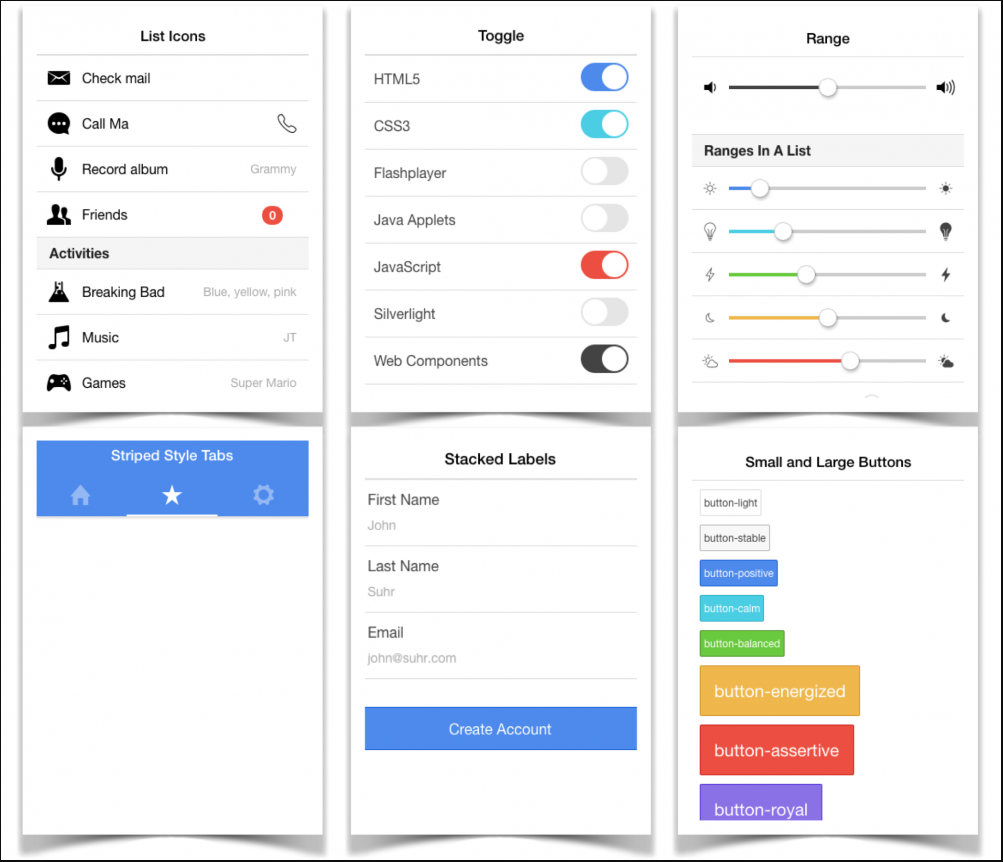
\includegraphics[width=10cm, height=7cm]{img/IonicUI.png}
\caption{Ionic UI.}
\end{figure}

\subsubsection{OS oriented styles}
Ionic is not just a good interface, it is adapted to the specifics of various operating systems and is thought through to the smallest detail. Animations, icons, fonts, all this with the same code will look like the operating system under which the application is built (Android or iOS, and starting with the second version and Windows Phone).\cite{IonicOS}

\subsection{Visual Studio Code}
\cite{mLab}.\\
\\
A sample of the MongoDB stucture is as follows\cite{WilliamZola}:
\begin{minted}{json}
{
    "_id" : 1

\end{minted}

\section{NoSQL database}
The ascent of Big Data made an interest for on a horizontally adaptable Data Management System. This prompted advancement of various types of Database Management System which all things considered go under NoSQL. NoSQL Databases are comprehensively separated into following sorts: Document, Key-value, Graph, Native object, Table type, Native XML and Hybrid Databases. All RDBMS databases depend on the same model, while, each of the NoSQL database takes after a distinctive model. NoSQL moves far from the robust institutionalized type of SQL database and empowers less complex information capacity arrangements. Therefore a NoSQL database is enhanced for the particular application.\cite{noSql}

\subsection{NoSql database types}

\begin{itemize}
\item Key-Value Storage \par
Key-Value Storages are straight forward and simple NoSQL frameworks, for example, Redis that are fundamentally a truly favour hash table. You have an esteem you need to get later, so you allocate it a key and in addition stuff it into the database, you can just inquiry a single object at any given moment and just by a single key.

\item Document Storage \par
Regularly, these are objects with a various levelled structure, for example, XML documents, JSON records, and some other kind of tree structure, yet the qualities of various nodes on the tree can be indexed. They have a much speed with respect to customary push construct SQL databases in light of query in light of the fact that they give up execution on joining. 

\item Columnar Storage  \par
These store the information in columns instead of lines, so refreshing and adding are costly, be that as it may, most questions are modest in light of the fact that each segment is basically certainly recorded. In any case, on the off chance that your inquiry can not utilize an index, you are in no better shape with a Columnar Store rather than a standard SQL database.

\item Graph Storage  \par
Diagram Databases (neo4j) make joins as shoddy as could be expected under the circumstances, on the grounds that even a straightforward row query would require many joins to recover. Tables can sort query would be slower than a standard SQL database in view of the greater part of the additional joins to retrieve the information. \cite{DataTypes}
\end{itemize}

\subsection{Advantages of NoSql}
NoSQL databases are very versatile, dependable, have a basic data model, amazingly exposed query language, no system for taking care of consistency and trustworthiness among data, and no help for security at the database level. A standout amongst the most vital points of interest of NoSQL databases is that the databases can handle unstructured information. Unstructured data can be word reports, messages, sound, video, or even interpersonal social network information. Too, NoSQL databases tend to scale extremely well on commodity equipment. Some even claim that NoSQL databases empower better execution, which is urgent for organizations with a lot of data. To empower quicker execution, NoSQL databases ordinarily don't cling to ACID (atomicity, consistency, isolation, durability) restrictions that are utilized as a part of relational databases. While this is recorded as a star for NoSQL as far as execution and processing time; we take note of that this likewise has unfortunate outcomes that will be tended to later. A case of NoSQL database's execution is Facebook's usage (Cassandra) that is equipped for dealing with more than 100 million clients persistently. \cite{AdvantagesnoSql}

\subsection{Examples of NoSQL}
\begin{itemize}
\item Key-Value Storage: \par
MUMPS, CouchDB, FoundationDB, Redis, Aerospike, Dynamo, MemcacheDB, Riak, OrientDB, Fair Com c-treeACE, Redis.

\item Apache CouchDB, MarkLogic, OrientDB, Clusterpoint, Couchbase, MongoDB.

\item Columnar Storage:  \par
Vertica, Cassandra, Hbase, Accumulo, Druid.

\item Graph Storage:  \par
Neo4J, OrientDB, Stardog, Allegro, InfiniteGraph, Virtuoso. 
\end{itemize}



\section{MongoDB}

\section{JQuery}

\section{JavaScript}
Javascript is a programming language with which web pages are given interactivity. It creates applications that are included in the HTML-code (for example, questionnaires or registration forms that are filled in by the user).\par The uniqueness of this programming language is that it is supported by almost all browsers and fully integrated with them, and all that can be done with it is done very simply. No other technology accommodates all these advantages together. To date, this technology is actively developing also developing a programming language Javascript2 \cite{JavaScript}

\begin{minted}{js}
// add two numbers
<script>
    var num1, num2, sum
    num1 = prompt("Enter first number")
    num2 = prompt("Enter second number")
    sum = parseInt(num1) + parseInt(num2) // "+" means "add"
    alert("Sum = " + sum)  // "+" means combine into a string
</script>
\end{minted}
\cite{JavaScriptCode}

\section{CSS}
CSS (Cascading Style Sheets) - cascading style sheets. In fact, they serve to separate the page structure and its content from its appearance.\par If the page is completely written in HTML, then each element of the code determines not only the content element of the page, but also its way of displaying. For example, not only that there is a text "Hello" in such and such a place, but also that this text is highlighted in bold and red.\par With the use of css code, everything happens a little differently. With the help of html, only the order of the content elements of the page and their classes are described. The corresponding classes are written in the css file. Each of them is assigned a set of properties. Now, when we assign a class to an html element, then all the properties of this class are applied to it. Do not write all these properties every time. Now, when sites have many pages, you can not do without css. \cite{CSS}

\begin{minted}{css}
body {
  font-family: Verdana, 
  Arial, sans-serif;
  }
\end{minted}

\chapter{System Design}

\begin{figure}[h]
\centering
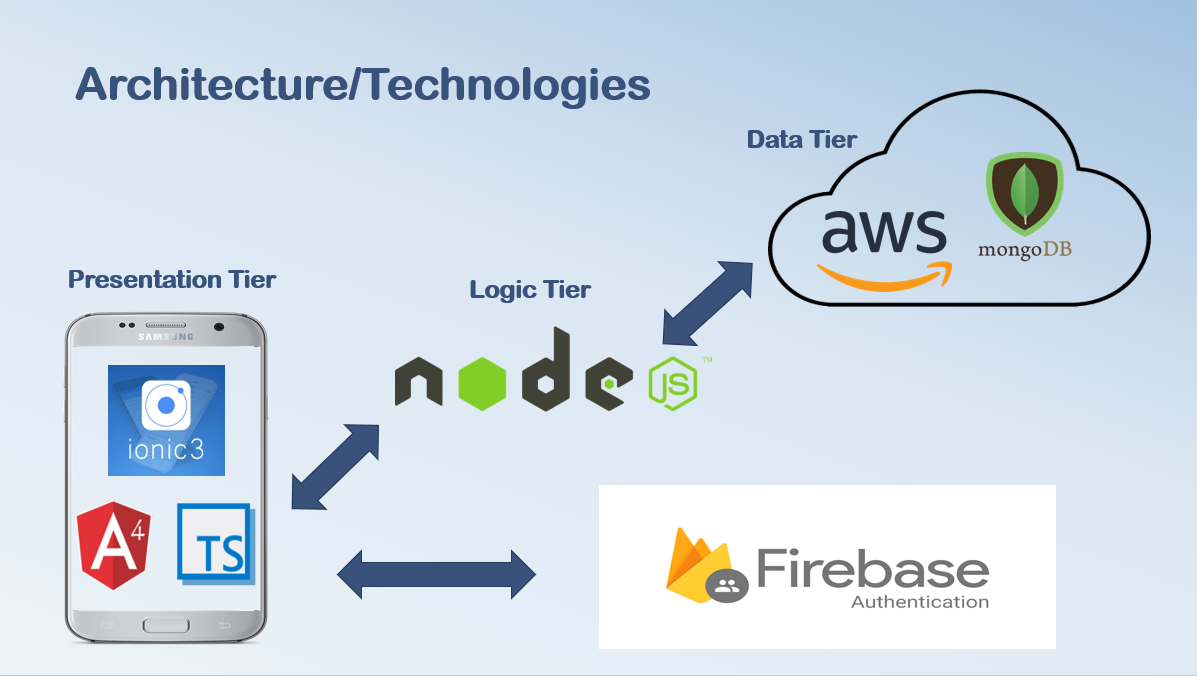
\includegraphics[width=14cm, height=7cm]{img/Architecture}
\caption{System Architecture.}
\end{figure}

\section{System Backend}

\subsection{Databases}
We chose databases..


\subsection{Security}

\section{Front End }

\subsection{Login/Register}
\par The login 

\begin{figure}[h]
\centering
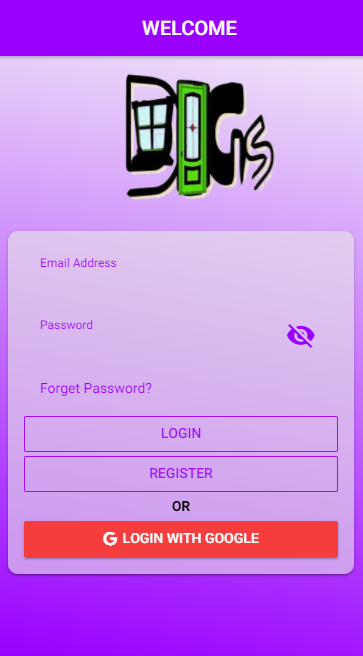
\includegraphics[width=8cm, height=16cm]{img/loginScreen}
\caption{Login Page}
\end{figure}

\subsection{Room page...}


\chapter{System Evaluation}
This Chapter evaluate the application
\begin{itemize}
    \item Scalability
    \item Robustness
    \item Maintainability
    \item Extensibility
\end{itemize}

\par \textbf{Scalability:} 

\par \textbf{Robustness:}.

\par \textbf{Maintainability:}

\par \textbf{Extensibility:} T

\section{Testing}

\section{Outcomes VS. Objectives}

\section{Limitations}

\section{Opportunities}

\chapter{Conclusion}


\begin{itemize}
\item A Test

\item A Test2
\item A Test3
\end{itemize}
A Test4
\section{Future Development}

\chapter{Appendix}

\textbf{Project Source Code Link: }link to github \\
\textbf{Project Documentation Link: } \\

